%package list
\documentclass{article}
\usepackage[top=3cm, bottom=3cm, outer=3cm, inner=3cm]{geometry}
\usepackage{graphicx}
\usepackage{url}
%\usepackage{cite}
\usepackage{hyperref}
\usepackage{array}
%\usepackage{multicol}
\newcolumntype{x}[1]{>{\centering\arraybackslash\hspace{0pt}}p{#1}}
\usepackage{natbib}
\usepackage{pdfpages}
\usepackage{multirow}
\usepackage{multirow}
\usepackage[T1]{fontenc}
\usepackage{imakeidx}
% Imagenes de costado
\usepackage{wrapfig}
\usepackage{graphicx}

% Modificar URLs
\usepackage{hyperref}
\hypersetup{
    colorlinks=true,
    linkcolor=black,
    filecolor=magenta,      
    urlcolor=blue,
    pdftitle={Overleaf Example},
    pdfpagemode=FullScreen,
    }

\urlstyle{same}


\usepackage[normalem]{ulem}
\useunder{\uline}{\ul}{}

\usepackage[newfloat]{minted}
\usepackage{caption}

\newenvironment{code}{\captionsetup{type=listing}}{}
\SetupFloatingEnvironment{listing}{name=Source Code}

% codigo fuente
\usepackage{listings}
\usepackage{color, colortbl}
\definecolor{dkgreen}{rgb}{0,0.6,0}
\definecolor{gray}{rgb}{0.5,0.5,0.5}
\definecolor{mauve}{rgb}{0.58,0,0.82}
\definecolor{codebackground}{rgb}{0.95, 0.95, 0.92}
\definecolor{tablebackground}{rgb}{0.0, 0.45, 0.63}
\lstset{frame=tb,
	language=bash,
	aboveskip=3mm,
	belowskip=3mm,
	showstringspaces=false,
	columns=flexible,
	basicstyle={\small\ttfamily},
	numbers=none,
	numberstyle=\tiny\color{gray},
	keywordstyle=\color{blue},
	commentstyle=\color{dkgreen},
	stringstyle=\color{mauve},
	breaklines=true,
	breakatwhitespace=true,
	tabsize=3,
	backgroundcolor= \color{codebackground},
}

%%%%%%%%%%%%%%%%%%%%%%%%%%%%%%%%%%%%%%%%%%%%%%%%%%%%%%%%%%%%%%%%%%%%%%%%%%%%
%%%%%%%%%%%%%%%%%%%%%%%%%%%%%%%%%%%%%%%%%%%%%%%%%%%%%%%%%%%%%%%%%%%%%%%%%%%%
\newcommand{\csemail}{@ulasalle.edu.pe}
\newcommand{\csdocente}{MSc. Maribel Molina Barriga}
\newcommand{\cscurso}{Sistemas Operativos}
\newcommand{\csuniversidad}{Universidad La Salle}
\newcommand{\csescuela}{Escuela Profesional de Ingeniería de Software}
\newcommand{\cspracnr}{04}
\newcommand{\cstema}{Planififcación de Procesos}
%%%%%%%%%%%%%%%%%%%%%%%%%%%%%%%%%%%%%%%%%%%%%%%%%%%%%%%%%%%%%%%%%%%%%%%%%%%%
%%%%%%%%%%%%%%%%%%%%%%%%%%%%%%%%%%%%%%%%%%%%%%%%%%%%%%%%%%%%%%%%%%%%%%%%%%%%


\usepackage[english,spanish]{babel}
\usepackage[utf8]{inputenc}
\AtBeginDocument{\selectlanguage{spanish}}
\renewcommand{\figurename}{Figura}
\renewcommand{\refname}{Referencias}
\renewcommand{\tablename}{Tabla} %esto no funciona cuando se usa babel
\AtBeginDocument{%
	\renewcommand\tablename{Tabla}
}

\usepackage{fancyhdr}
\pagestyle{fancy}
\fancyhf{}
\setlength{\headheight}{30pt}
\renewcommand{\headrulewidth}{1pt}
\renewcommand{\footrulewidth}{1pt}
\fancyhead[L]{\raisebox{-0.2\height}{
\includegraphics[width=3cm]{logo_ulasalle (1).png}}}
\fancyhead[C]{}
\fancyhead[R]{\fontsize{7}{7}\selectfont	\csuniversidad \\ \csescuela \\ \textbf{\cscurso} }
\fancyfoot[L]{}
\fancyfoot[C]{Sistemas Operativos}
\fancyfoot[R]{Página \thepage}



\begin{document}

	\vspace*{10px}
	
	\begin{center}	
		\fontsize{17}{17} \textbf{ Práctica \cspracnr}
	\end{center}
	%\centerline{\textbf{\underline{\Large Título: Informe de revisión del estado del arte}}}
	%\vspace*{0.5cm}
	

\renewcommand{\arraystretch}{1.5}
\begin{table}[h]
	\begin{tabular}{|x{4.7cm}|x{4.8cm}|x{4.8cm}|}
		\hline 
		\textbf{DOCENTE} & \textbf{CARRERA}  & \textbf{CURSO}   \\
		\hline 
		\csdocente & \csescuela & \cscurso    \\
		\hline 
	\end{tabular}
\end{table}	

\begin{table}[h]
	\begin{tabular}{|x{4.7cm}|x{4.8cm}|x{4.8cm}|}
		\hline 
		\textbf{GRUPO} & \textbf{TEMA}  & \textbf{DURACIÓN}   \\
		\hline 
		\ 6 & \cstema & 5 horas   \\
		\hline 
	\end{tabular}
\end{table}
\renewcommand{\arraystretch}{1} 
	\section*{Integrantes}
	 	\begin{itemize}
            \item José Carlos Machaca Vera
	 		\item Jhosep Alonso Mollapaza Morocco
	 		\item Patrick Andres Ramirez Santos
	 \end{itemize}
 
	\tableofcontents


	
	\newpage

\section{Actividades}
\subsection{Actividad 1}
Este código imprime los identificadores del proceso en ejecución (PID) y
su proceso padre (PPID). Se refleja la gestión de procesos, donde cada 
nuevo proceso se crea a partir de otro existente (proceso padre) y 
recibe un PID único. Al observar el PID y PPID, se puede entender la 
estructura jerárquica del sistema operativo, además de que cada nuevo 
proceso se crea a partir de otro existente y recibe un PID único, donde
cada proceso tiene un lugar específico en el árbol de procesos,
iniciando desde el proceso INIT.
\begin{code}
	\captionof{listing}{Actividades/e1.c}
	\inputminted{c}{../Actividades/e1.c}
\end{code}
\begin{figure}[h]
	\caption{Compilación y ejecución de Actividad 1}
	\centering
	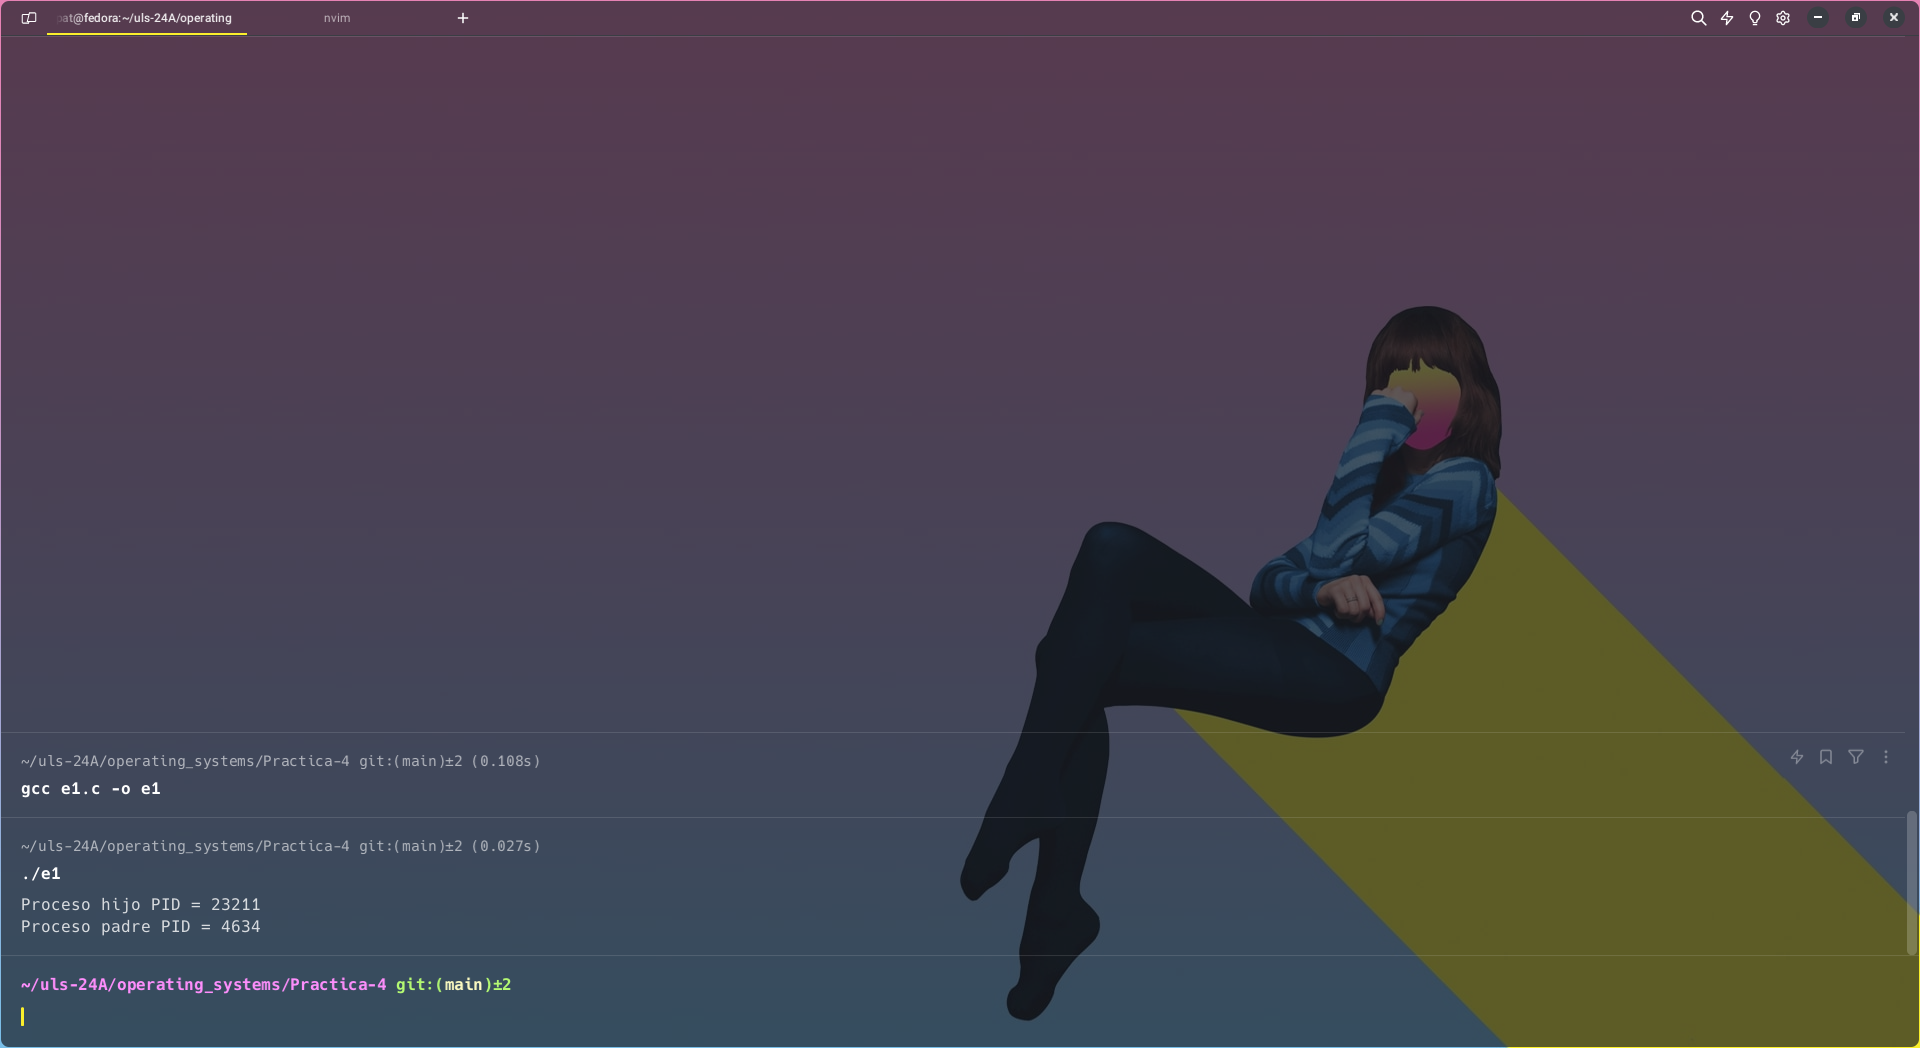
\includegraphics[scale=0.3,trim={0 0 20cm 25cm},clip]{act-e1.png}
\end{figure}


\subsection{Actividad 2}
Analisamos el código y respondemos las siguientes preguntas ¿cuántos 
procesos se crean?, ¿qué realiza cada uno de estos procesos?, ¿existe 
algún tipo de relación entre estos procesos?.
    \begin{itemize}
        \item Creación de procesos: Se crean 2 procesos, el proceso 
		principal (padre) y un proceso hijo. "pid\_t pid\_hijo;" 
		"pid\_hijo = fork();"
        \item Función de los procesos: El Proceso padre Invoca la 
		función crear(), llama a fork() para crear un proceso hijo 
		y luego espera 20 segundos antes de terminar. Y el proceso 
		hijo ejecuta el comando ls -lh / para listar los archivos 
		y directorios en el directorio raíz usando execv(). Si execv()
		 falla, imprime un error y aborta.
        \item Relación entre los procesos: Sí, existe una relación 
		padre-hijo entre los procesos. El proceso padre crea el 
		proceso hijo mediante fork() y mantiene un breve control 
		sobre él mediante la espera de 20 segundos antes de terminar 
		su ejecución.
	\end{itemize}
	\begin{code}
		\captionof{listing}{Actividades/e2.c}
		\inputminted{c}{../Actividades/e2.c}
	\end{code}
	\begin{figure}[h]
		\caption{Compilación y ejecución de Actividad 2}
		\centering
		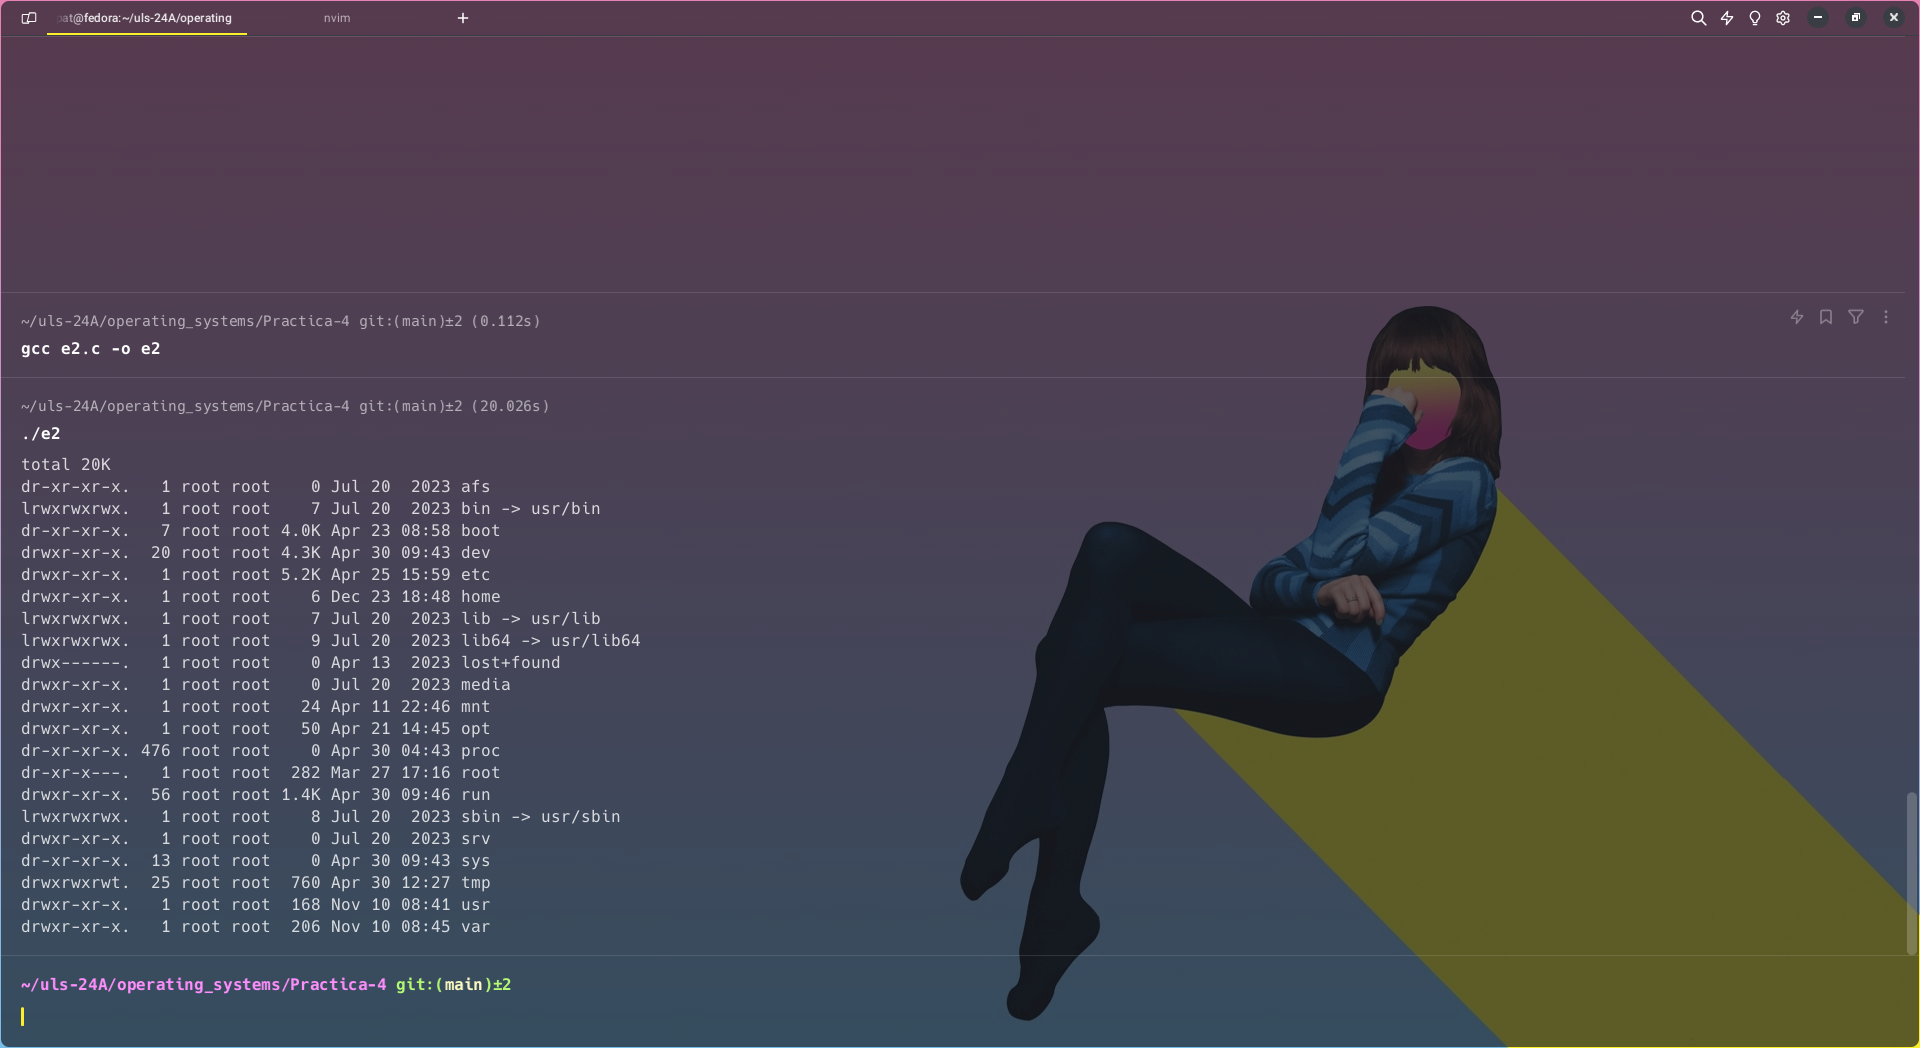
\includegraphics[scale=0.3,trim={0 0 20cm 10cm},clip]{act-e2.png}
	\end{figure}

\section{Ejercicios}
\subsection{Ejercicio 1}
El comportamiento del código es que el proceso hijo modifica una copia
local de la variable value, y el proceso padre conserva el valor 
original de value porque fork() crea un espacio de memoria separado 
para el hijo. Por eso, el valor impreso por el padre sigue siendo 5.
\begin{code}
	\captionof{listing}{Ejercicios/e1.c}
	\inputminted{c}{../Ejercicios/e1.c}
\end{code}

\begin{figure}[h]
\caption{Compilación y ejecución de Ejercicio 1}
\centering
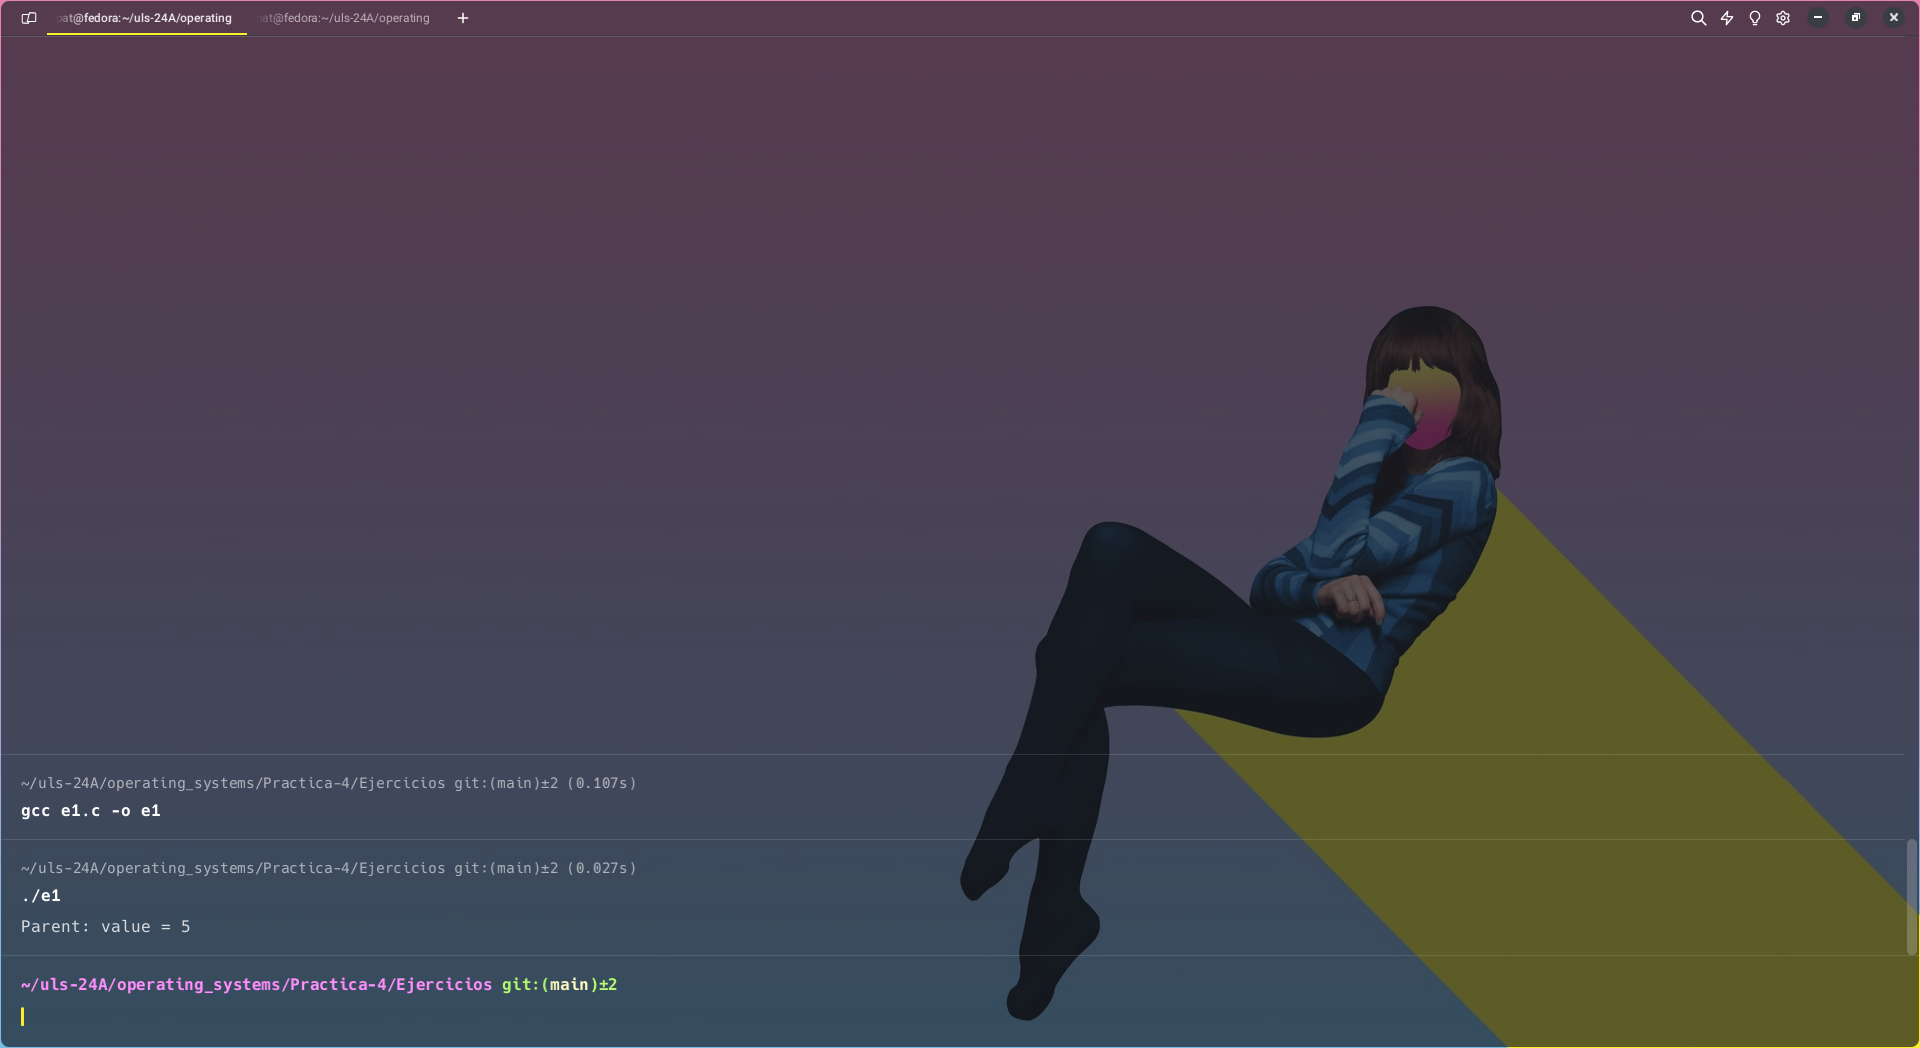
\includegraphics[scale=0.3,trim={0 0 20cm 25cm},clip]{ejer-e1.png}  
\end{figure}

\subsection{Ejercicio 2}
Código ejecutado por el proceso padre: El proceso padre espera a que 
el proceso hijo termine su ejecución con wait(NULL). Una vez que el 
hijo ha completado su tarea y ha terminado, el padre procede a imprimir
"Child completado". Esto indica que el padre ha detectado la 
finalización del hijo.
\begin{minted}{c}
	else {
    	wait(NULL);
    	printf("Child completado");	
	}
\end{minted}


Código ejecutado por el proceso hijo: El proceso hijo ejecuta el 
comando ls para listar el contenido del directorio actual usando 
execlp(), una función que reemplaza la imagen del proceso actual 
con un nuevo programa. Aquí, el proceso hijo efectivamente se convierte
en el proceso del comando ls.
\begin{minted}{c}
	else if (pid == 0) {
    execlp("/bin/ls", "ls", NULL);
	}
\end{minted}

\begin{code}
	\captionof{listing}{Ejercicios/e2.c}
	\inputminted{c}{../Ejercicios/e2.c}
\end{code}
\begin{figure}[h]
	\caption{Compilación y ejecución de Ejercicio 2}
	\centering
	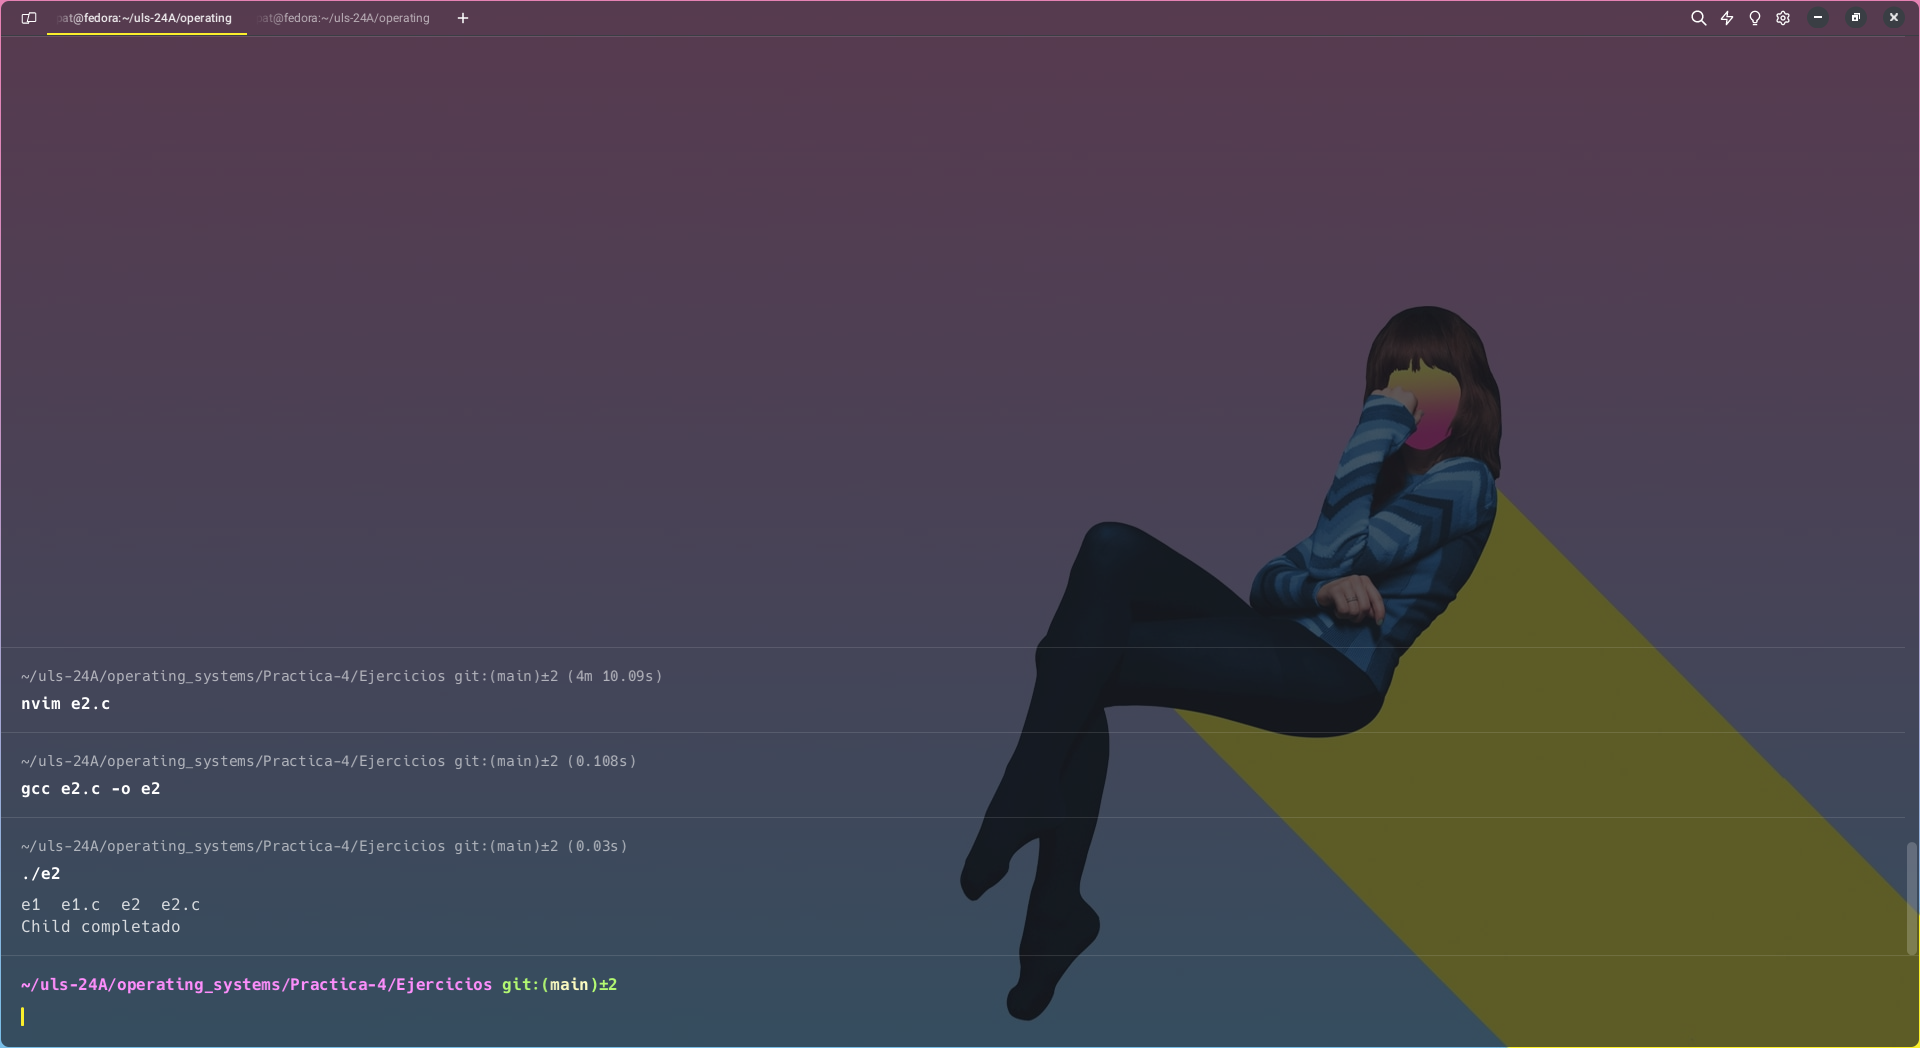
\includegraphics[scale=0.3,trim={0 0 20cm 26cm},clip]{ejer-e2.png}
\end{figure}

\newpage
\subsection{Ejercicio 3}
\subsubsection*{Inicio del proceso padre}
    \begin{itemize}
        \item Imprime que inicialmente hay un solo proceso.
        \item Realiza la primera llamada a fork() para crear el primer
		 hijo.
	\end{itemize}
\subsubsection*{Primer hijo (HIJO 1)}
    \begin{itemize}
        \item Imprime un saludo y menciona que se detendrá por 20 
		segundos (aunque en el código dice 5s, en realidad son 20).
        \item Se suspende con sleep(20) y luego termina.
	\end{itemize}
\subsubsection*{Proceso padre (continuación)}
    \begin{itemize}
        \item Después de crear el primer hijo, imprime el PID del 
		primer hijo.
        \item Realiza otra llamada a fork() para crear el segundo hijo.
	\end{itemize}
\subsubsection*{Segundo hijo (HIJO 2)}
    \begin{itemize}
        \item Imprime un saludo y anuncia que ejecutará el comando ls.
        \item Ejecuta execlp("ls", "ls", NULL) para listar los 
		directorios. Si execlp() falla, imprime un mensaje de error.
	\end{itemize}
\subsubsection*{Proceso padre (finalización)}
    \begin{itemize}
        \item Después de crear ambos hijos, imprime el PID del segundo 
		hijo.
        \item Anuncia que esperará a que ambos hijos terminen. Utiliza 
		wait(NULL) dos veces para esperar que cada hijo termine, 
		imprimiendo el PID de cada hijo que termina.
	\end{itemize}
\begin{code}
	\captionof{listing}{Ejercicios/e3.c}
	\inputminted{c}{../Ejercicios/e3.c}
\end{code}
\begin{figure}[h]
	\caption{Compilación y ejecución de Ejercicio 3}
	\centering
	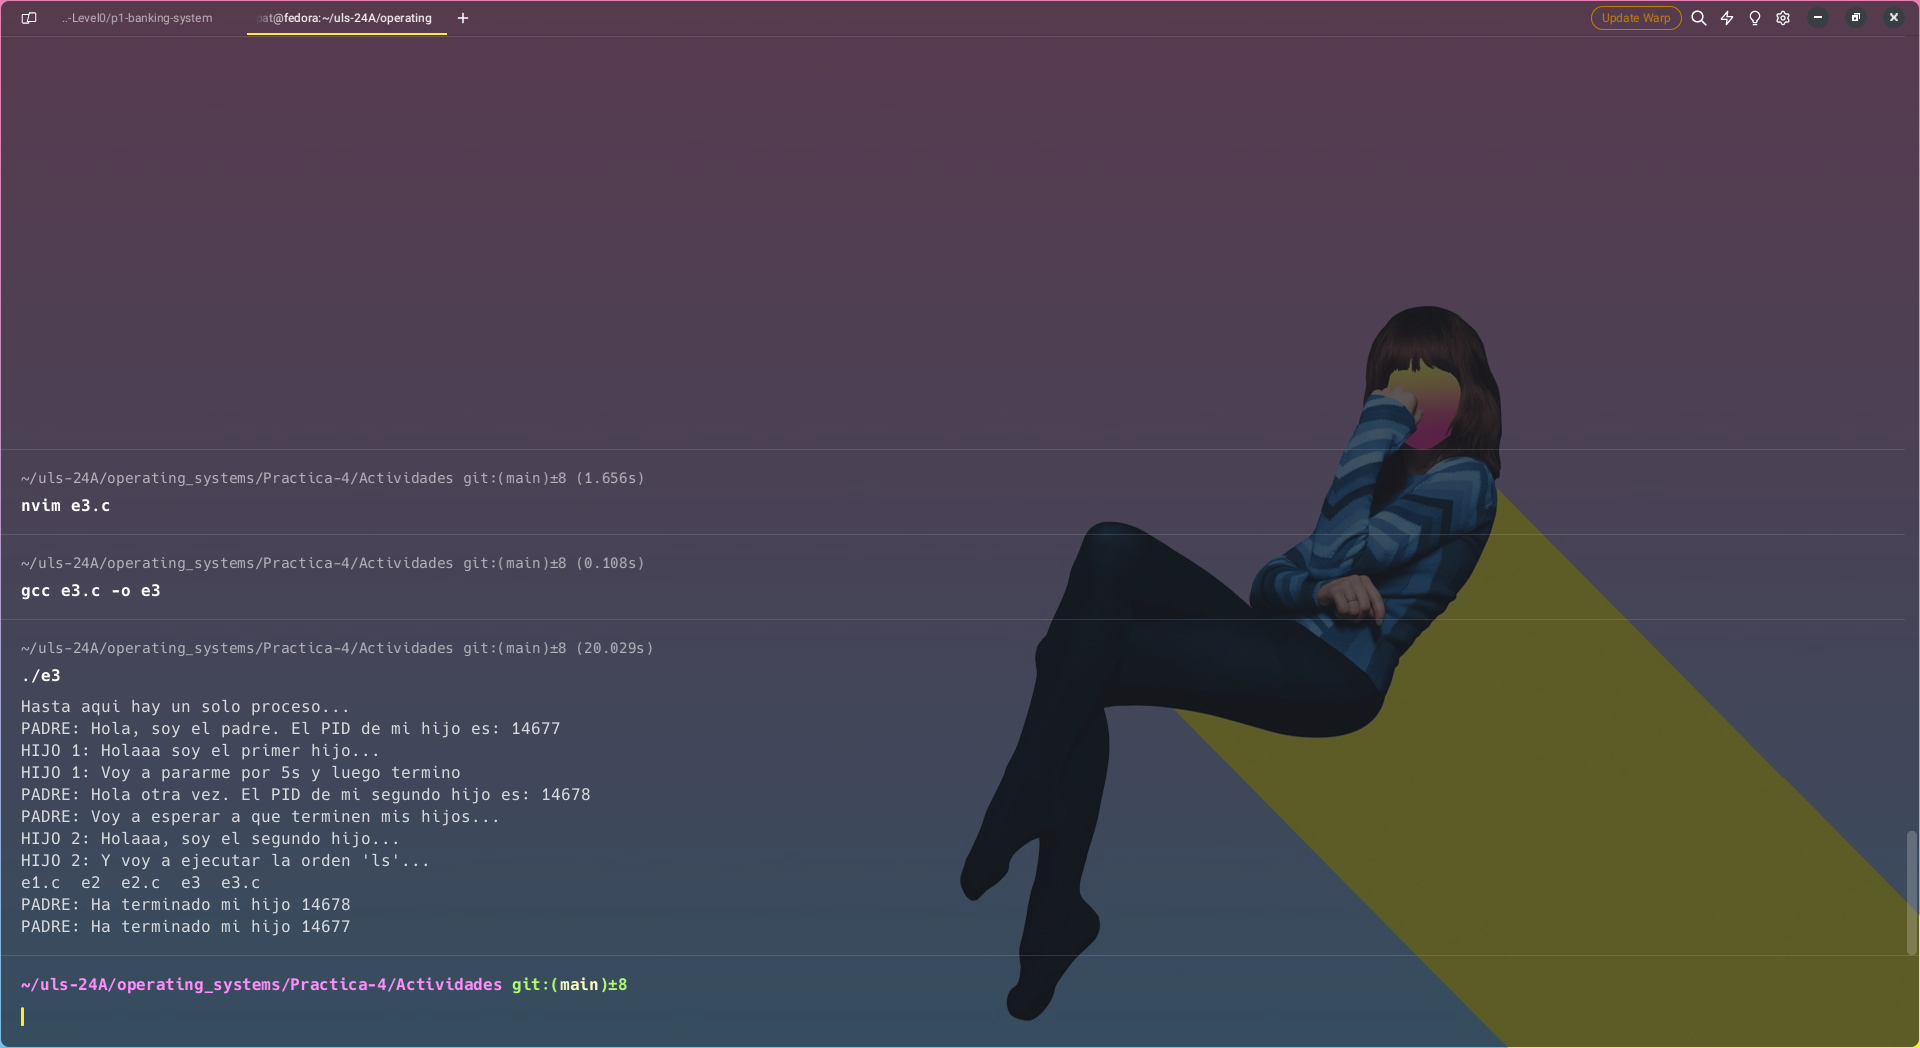
\includegraphics[scale=0.3,trim={0 0 20cm 18cm},clip]{ejer-e3.png}
\end{figure}

\subsection{Ejercicio 4}
Después de las tres llamadas a fork(), hay un total de 8 procesos 
generados. Este resultado es una consecuencia del crecimiento 
exponencial donde cada fork() duplica el número de procesos actuales.
\begin{code}
	\captionof{listing}{Ejercicios/e4.c}
	\inputminted{c}{../Ejercicios/e4.c}
\end{code}
\begin{figure}[h]
	\caption{Compilación y ejecución de Ejercicio 4}
	\centering
	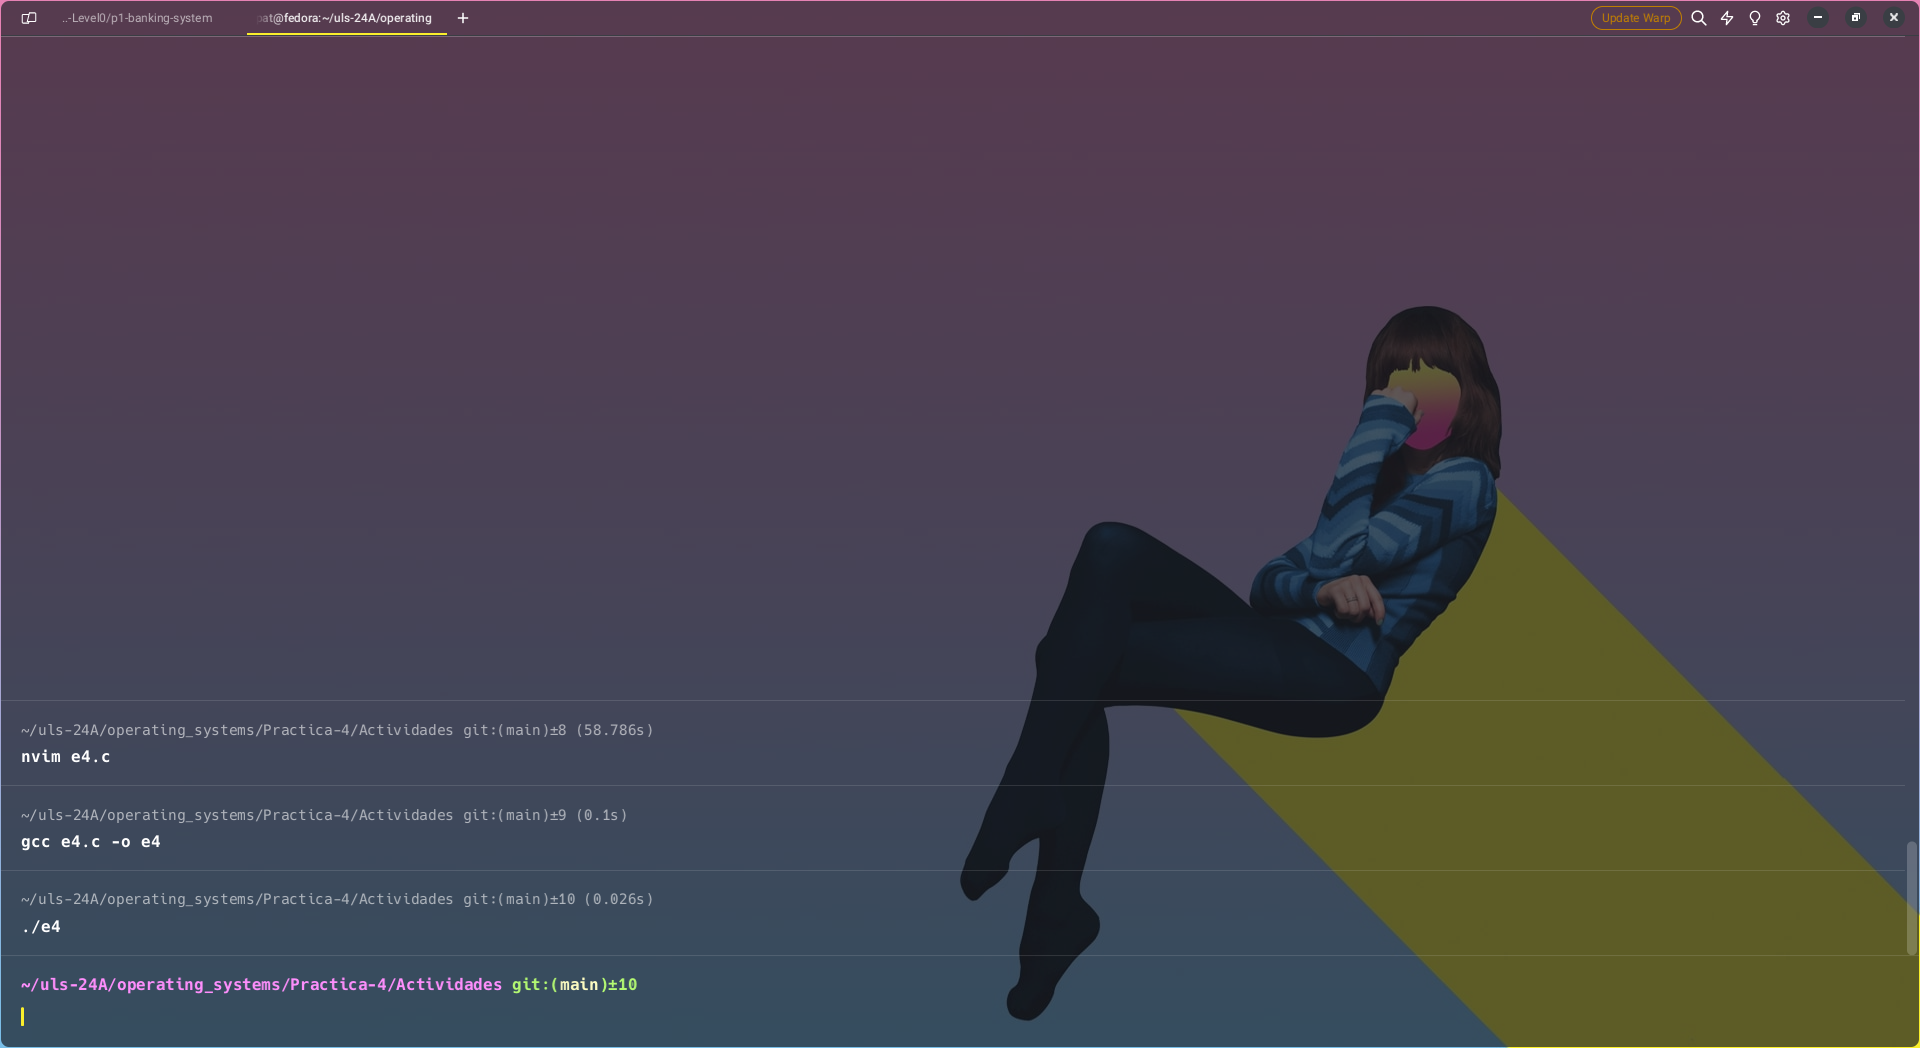
\includegraphics[scale=0.3,trim={0 0 20cm 26cm},clip]{ejer-e4.png}
\end{figure}

\subsection{Ejercicio 5}
\subsubsection*{Funciones que permiten compartir memoria}
    \begin{itemize}
        \item shm\_open: Esta función crea o abre un objeto de memoria
		compartida. En el código del productor, se usa con los flags
		O\_CREAT | O\_RDWR para crear el objeto si no existe y 
		permitir lectura y escritura. En el código del consumidor, 
		se abre con O\_RDONLY para solo lectura.
        \item ftruncate: Usada por el productor para establecer el 
		tamaño del objeto de memoria compartida. En este caso, se 
		establece a SIZE, que es 4096 bytes.
        \item mmap: Mapea el objeto de memoria compartida en el espacio 
		de direcciones del proceso. En el productor, se configura con 
		PROT\_WRITE para permitir escritura y en el consumidor con 
		PROT\_READ para solo lectura, ambos usando MAP\_SHARED para 
		permitir que los cambios sean visibles entre procesos.
        \item shm\_unlink: Utilizada por el consumidor para desvincular 
		el objeto de memoria compartida, lo que indica que el nombre 
		puede ser reutilizado y el objeto será eliminado una vez que 
		todos los procesos que lo tienen abierto lo cierren.
	\end{itemize}

	El codigo se compiló y ejecutó con los siguientes comandos:
	\begin{minted}{bash}
		$ gcc -lrt productor.c -o productor
		$ gcc -lrt consumidor.c -o consumidor
		$ ./productor && ./consumidor
	\end{minted}

	\begin{code}
		\captionof{listing}{Ejercicios/producer.c}
		\inputminted{c}{../Ejercicios/producer.c}
	\end{code}
	\begin{code}
		\captionof{listing}{Ejercicios/consumer.c}
		\inputminted{c}{../Ejercicios/consumer.c}
	\end{code}

	\begin{figure}[h]
		\caption{Compilación y ejecución de Ejercicio 5}
		\centering
		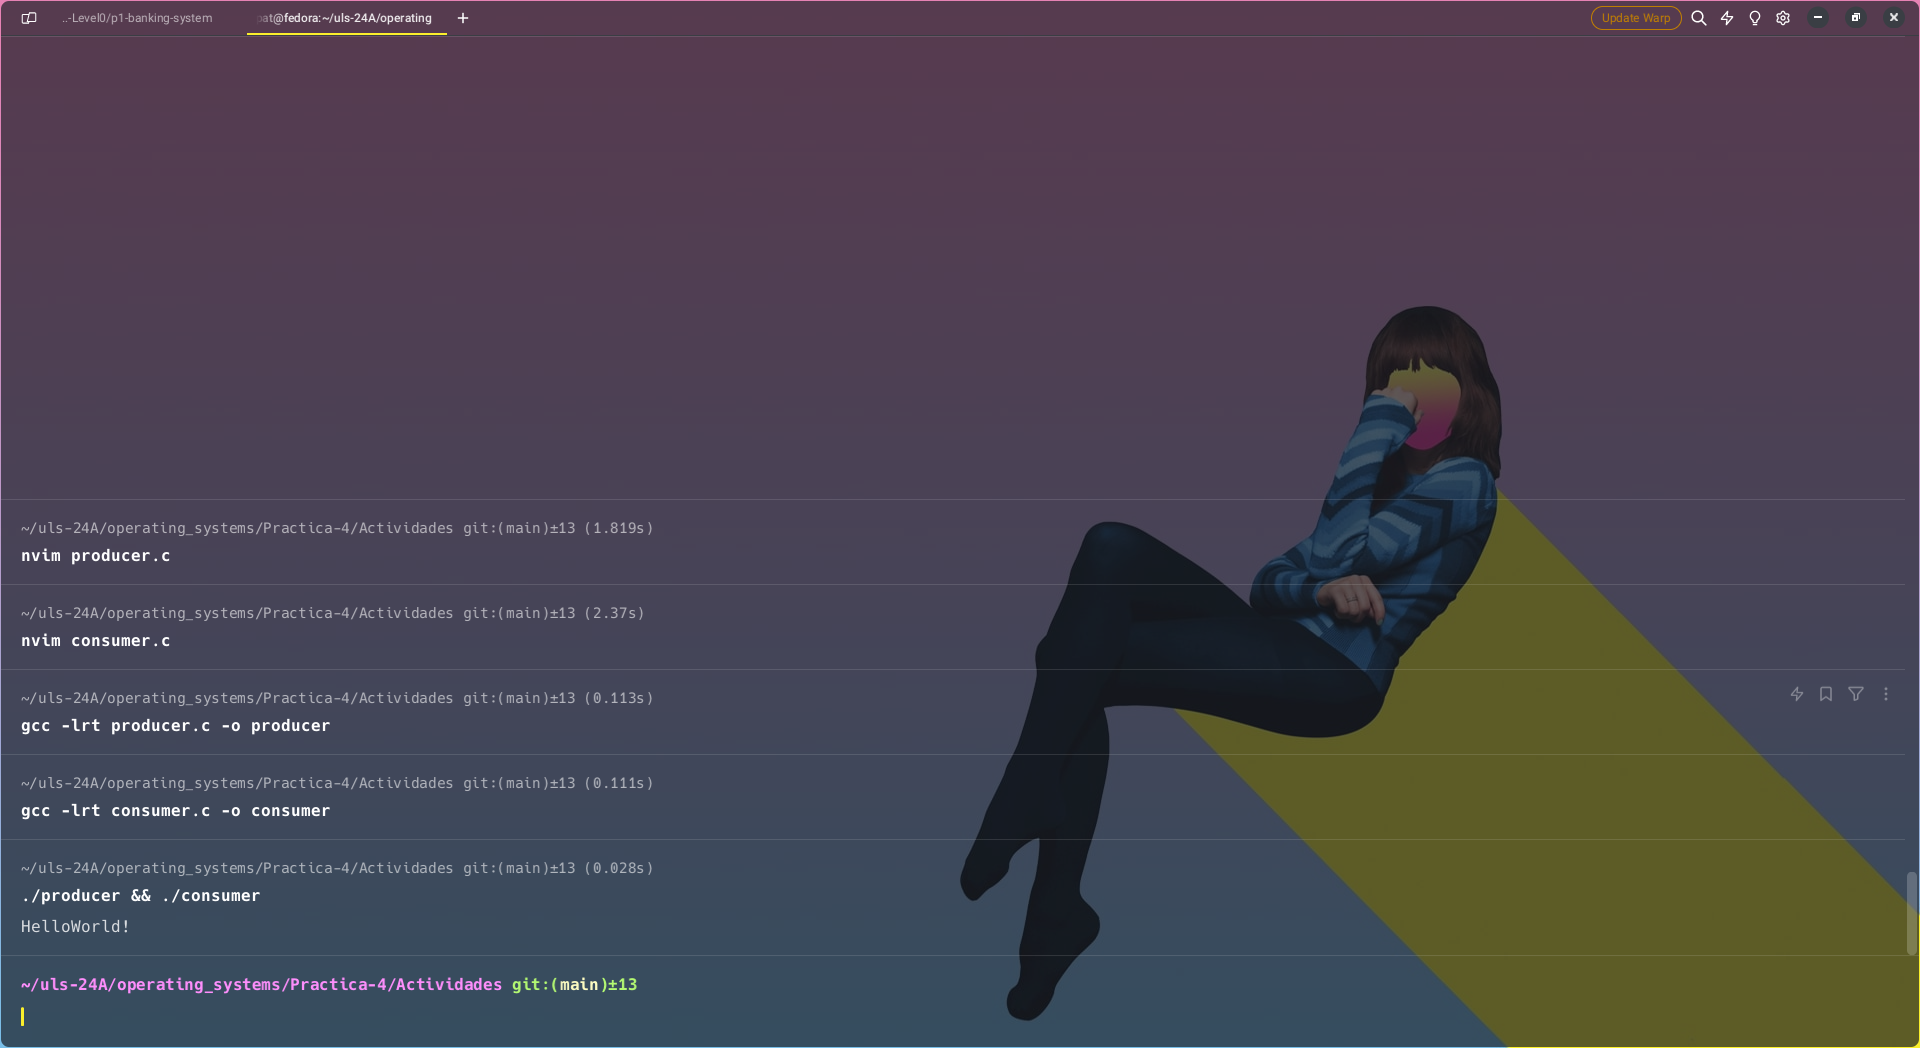
\includegraphics[scale=0.3,trim={0 0 20cm 26cm},clip]{ejer-e5.png}
	\end{figure}

\newpage

\section{Cuestionario}
    \begin{enumerate}
        \item La principal característica de fork es que crea una
		copia exacta del proceso llamante (padre) en un nuevo proceso 
		(hijo). El proceso hijo recibe una copia del espacio de memoria 
		del padre pero con su propio espacio de direcciones. Esto 
		significa que cualquier cambio realizado en el espacio de 
		memoria del hijo no afecta al padre, y viceversa.
        \item En sí, puedes crear tantos procesos hijos como lo permitan 
		los recursos del sistema, pero en la práctica, hay límites 
		establecidos por el sistema operativo. Estos límites pueden 
		incluir el número máximo de procesos por usuario o límites 
		globales de procesos, que se pueden consultar con comandos como 
		'ulimit -u' en sistemas tipo Unix/Linux.
        \item 'execlp' es una función que ejecuta un programa, 
		reemplazando la imagen del proceso actual con un nuevo programa. 
		Utiliza el PATH del sistema para buscar el ejecutable especificado 
		si no se da una ruta completa. Por ejemplo, 
		execlp("ls", "ls", "-l", NULL); ejecutaría el comando 'ls -l', 
		listando archivos en el directorio actual con detalles
        \item Este código crea procesos para simular el grafo de 
		precedencia de la figura, asegurando que los mensajes se 
		impriman en el orden correcto de acuerdo con las dependencias 
		del grafo
        \begin{code}
			\captionof{listing}{Implementación del grafo}
			\inputminted{c}{../Cuestionario/cuestionario.c}
		\end{code}
		\begin{figure}[h]
			\caption{Compilación y ejecución del grafo}
			\centering
			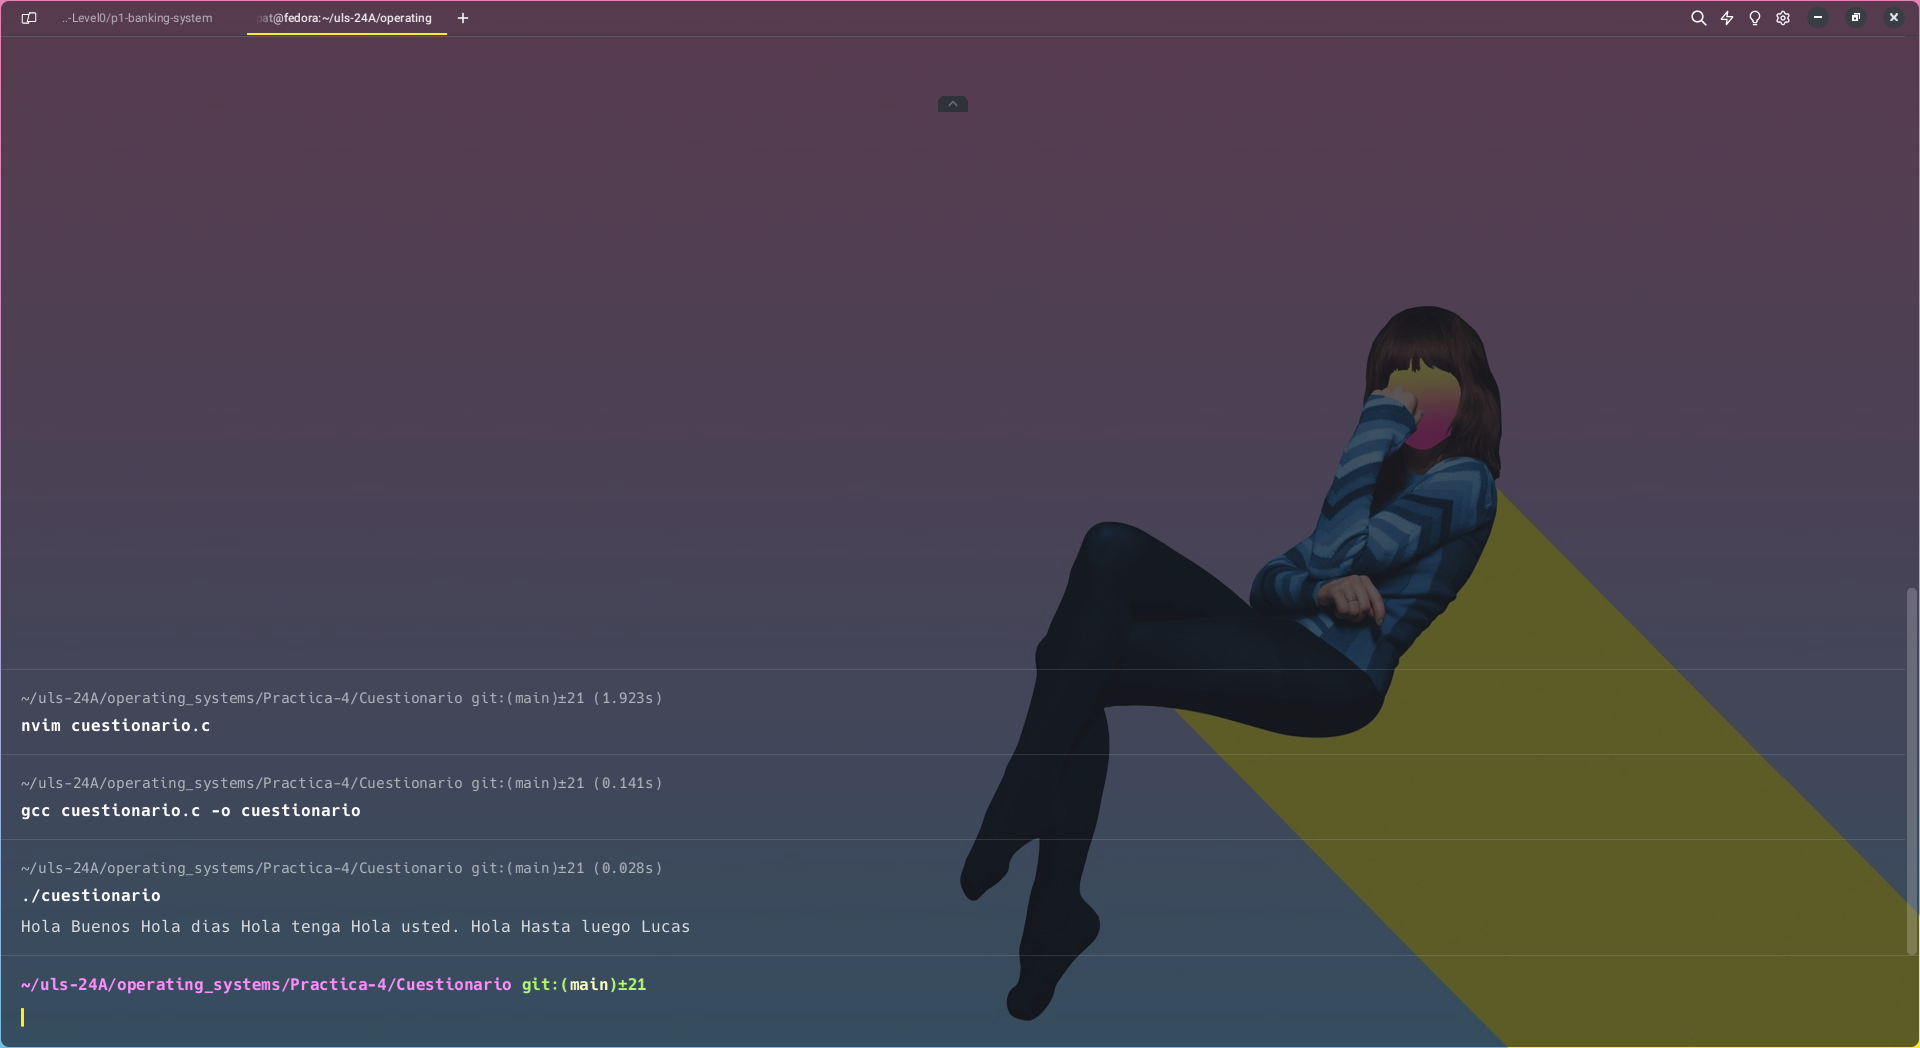
\includegraphics[scale=0.3,trim={0 0 20cm 26cm},clip]{cuestionario.png}
		\end{figure}
	\end{enumerate}

\newpage
\renewcommand{\listlistingname}{Indice Source Code}
\listoflistings
\addcontentsline{toc}{section}{\listlistingname}

\renewcommand{\listfigurename}{Indice de Capturas de Pantalla}
\listoffigures 
\addcontentsline{toc}{section}{\listfigurename} 

\end{document}
